% 
%  chapter2.tex
%  ThesisISEL
%  
%  Created by Matilde Pós-de-Mina Pato on 2012/10/09.
%
\chapter{Background and State of the Art}
\label{cha:users_manual}

Firstly, on section \ref{sec:related_work}, will be made an overview on previously developted work made on this subject, then, on section \ref{sec:async_concepts}, will be made a characterization of the key concepts related to it. By last, on section \ref{sec:state_of_the_art}, are presented and explained several technologies representative of the state of the Art on asynchronous data sequencing in different programming realities, e.g. on Kotlin, JAVA and C\#. 


% ================
% = Related work =
% ================
\section{Related Work} % (fold)
\label{sec:related_work}

% Initially, when computers had a single processing unit, the networks only allowed the exchange of few bytes per second and the data servers didn't had the responsiveness requirements that are mandatory today; software computational systems were simpler, in the sense that operations were mostly made in a single execution thread. 
% The servers design, were made without many concerns about availability under demand pressure or computer resource optimization. 
% Consequently, operations that required intensive IO interactions or data request from an external sources, were mostly blocking, non-flexible in terms of responsiveness and interoperability. 

From the end of 80´s to the beginning of the 2000´s, with the acceleration of Moores´s Law in hardware and network bandwidth development, the creation of the web as we know today through the wide spread of use of the HTTP protocol and the support from new operative systems with multithreading support, the nescessity of high responsivness servers started to grow. This increase in demand of new ways to handle data through paralelism, caused the nescessity of design new programming models compatible with concurrent work. 

One of the earlier advances made in this subject is the introduction to the \texttt{Proctor Pattern} in a paper made in 1997 by Tim Harrison, Irfan Pyarali, Douglas C. Schmidt and Thomas D.Jordan. 
In the paper, are identified four properties that high-performance web server must have: 
\begin{itemize}
	\item Concurrency - The server must process multiple client requests simultaneously.\\
	\item Efficiency - The software design must be built aiming the use of least hardware resources as possible. \\
	\item Simplicity - The code of the solution must be easy to understand, modular and avoid own built design patterns as possible. \\
    \item Adaptability - The system must be totally decoupled from client implementations, allowing it to be easily used by any client independently of the underlying technologic realities. To achieve this, may be used standards e.g. REST or SOAP.\\
\end{itemize}

The authors propose the \texttt{Proactor Pattern}, because in their opinion, conventional concurrency models fail to fully achieve the enumerated properties. In the paper, before presenting the \texttt{Proactor Pattern}, are identified two major concurrency models, namely: multithreading and reactive event dispatching. 

The paper refers that one of the most direct implementations of the multithreading approach, is the handling of multiple requests by creating a new thread every time. Each request will them be fully processed and the recently  created thread is them be disposed after the work is finished. 
This solution has several serious issues; firstly, creating a new thread per request is highly costly in term of computional resources,
because are involved context switches between user and kernel modes; secondly, must be taken in account synchronization to maintain data integrity. 
On last, if the server receives a high demand of requests, the server easily blocks in the process of creating and disposing threads. 
To avoid this issue, the authors, recommended the use of dynamic threadpools to process requests, where each request will be linked to a pre-existing thread, avoiding all the overhead of creating and disposing a thread per request;
however, by the authors, synchronization complexity maintains.

Another traditional concurrency model identified by the authors of the paper, is \texttt{Reactive Synchronous Event Dispatching}. 
In this model, a \texttt{Reactor}, with a single thread in a loop, is constantly listening requests from clients and sending work requests to an entity named \texttt{Handler}. 
The \texttt{Handler} will then process the IO work Synchronously and register a connection in the \texttt{Reactor}. When the connection becomes available for writing, the \texttt{Reactor} notifies the \texttt{Handler} to asynchronously send the data that is being obtained through IO operations to the client.\\
The authors identify several drawbacks with this approach: the code for this approach is complex, since is following a single thread approach to process requests. If a request processing blocks for any reason, can exist an impact in the processing of another requests and impact the readiness of the whole system. 
Another issue with this approach, is from the fact that the \texttt{Handler} makes a read from a data source e.g a file in a file system, and brings that data to memory. The question that arises from this is: What happens when the data obtained through IO becomes greater than the memory can hold and a sending to the client is slower that a reading made by OS IO mechanisms!?

To mitigate these issues, is suggested the \texttt{Proactor Pattern}. This pattern is very similar to the \texttt{Reactive Synchronous Event Dispatching}, however, after the requests are accepted, the IO work is dispatched asynchronously to the underlying OS IO subsystem. 
To retrieve the result, is previously registered a callback in a module named \texttt{Completion Handler}. The callback will be called when the IO operations end, to asynchronously send the data to the client. 
This model \texttt{Proactor Pattern} design creates the ground for the building of modern models, e.g. \texttt{Tasks}, \texttt{CompletableFutures} and \texttt{Javascript callback model}. //todo This motivated the writing of the  papers of : .... 


\begin{figure}[ht]
	\centering
	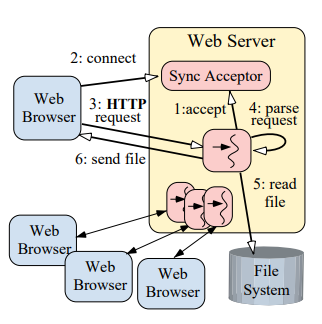
\includegraphics[width=0.65\textwidth]{alternative_1}
	  \caption{Multithreading solution example}
  \label{fig:bibtex}
\end{figure}


\begin{figure}[ht]
	\centering
	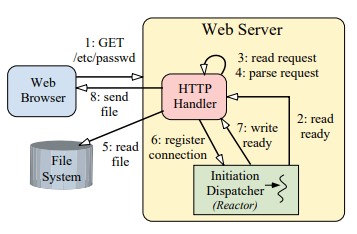
\includegraphics[width=0.65\textwidth]{alternative_2}
	  \caption{Dispatcher example}
  \label{fig:bibtex}
\end{figure}

\begin{figure}[ht]
	\centering
	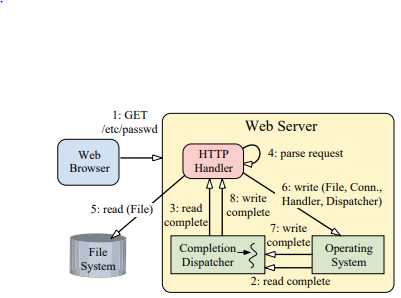
\includegraphics[width=0.65\textwidth]{alternative_3}
	  \caption{Proactor example}
  \label{fig:bibtex}
\end{figure}

% section introduction (end)

% ====================
% = Folder Structure =
% ====================
\section{Asynchronous sequencing key concepts and design alternatives} % (fold)
\label{sec:async_concepts}

With the development of several approaches and implementations related to asynchronous data sequencing in several programming plataforms; a dictionary
of properties, concepts and design alternatives started to grow by itself. In the following, are discussed several of the concepts related with asynchronous data sequencing, namely:


\begin{itemize}
	\item Synchronous vs Asynchronous - Before explaining more terms related with asynchronous data sequencing, its important to clarify what is an asynchronous call in programming. An asynchronous call, is a call to a function or routine with imediatte return, where the result of that processing is may be done outside of the main programm time sequence.  
	%For examples, a call to the function \texttt{ x(input, callback)}, return immediately, however, the processing is done outside of the time scope of the caller. 
	%Add Sync vs Async 
	
	\item Callbacks - In terms of asynchronous.\\
	\item Tasks - . \\
	\item Cancelables - . \\
	\item Error Handling - \\
	\item Intrisic Words - \\
	\item Push vs Pull - \\
	\item Streams -  \\
	\item Hot vs Cold -\\
	\item Reactive Streams - \\
	\item Async Enumerables - \\ 

    
\end{itemize}

% The template file for writing dissertations in  \texttt{LaTeX} is organized into a main directory, a set of files and sub-directories:
% \begin{enumerate}
% 	\item[ThesisISEL] This is the main directory and includes:
% 	\begin{enumerate}
% 		\item \textbf{Logo} Directory with Faculty logos;
% 		\item \textbf{sty} Directory will all sty files that help in formatting document;
% 		\item \textbf{Chapters} Directory where to put user files (text and figures);
% 		\begin{enumerate}
% 		\item \textbf{scripts} Directory with useful bash scripts, e.g., for cleaning all temporary files;
% 		\item \textbf{img} Directory with all images of your thesis;
% 		\end{enumerate}
% 		\item \textbf{alpha-pt.bst} A file with bibliography names in portuguese, e.g., 'Relatório Técnico' e 'Tese de Mestrado' instead of 'Technical Report' and 'Master Thesis'. This file is used automatically if Portuguese is selected as the main language (see below);
% 		\item \textbf{defaults.tex} A file with the main default values for the package (institution name, faculty's logo, degree name and similars);
% 		\item \textbf{personaldataofthesis.tex} A file with the main default values for the package (identification of report as well as the author and juries);
% 		\item \textbf{template.tex} The main file. You should run  \texttt{LaTeX} in this one. Please refrain from changing the file content outside of the well defined area;
% 		\item \textbf{bibliography.bib} The bib file. An easy way to find to import citation into \texttt{bibtex} is select option \texttt{Show links to import citation into
% Bib\-Tex} in \href{http://scholar.google.pt/scholar_settings?hl=en&as_sdt=0,5}{\texttt{Scholar google settings}}.
% 		\item \textbf{thesisisel.cls} The  \texttt{LaTeX} class file for the thesis{} style. Currently, some of the defaults are stored here instead of \verb!defaults.tex!. This file should not be changed, unless you're ready to play with fire! :)
% 	\end{enumerate}
% \end{enumerate}

% Again, we would like to recall that all the user \texttt{LaTeX} files should be stored in the \verb!ThesisISEL! directory, and all the images in \verb!ThesisISEL/Chapters/img! directory.\todo[inline]{Yet another note!}
% section folder_structure (end)

% ===================
% = Package options =
% ===================
\section{State of the Art} % (fold)
\label{sec:state_of_the_art}

The thesis{} style includes the following options, that must be included in the options list in the \verb!\documentclass[options]{thesisisel}! line at the top of the \texttt{template.tex} file.

The list below aggregates related options in a single item. For each list, the default value is prefixed with a *.

\subsection{Language Related Options} % (fold)
\label{sub:language_related_options}

You must choose the main language for the document. The available options are:

\begin{enumerate}
	\item \textbf{*pt} --- The text is written in Portuguese (with a small abstract in English).
	\item \textbf{en} --- The text is written in English (with a small abstract in Portuguese).
\end{enumerate}

The language option affects:
\begin{itemize}
	\item \textbf{The order of the summaries.} At first the abstract in the main language and then in the foreign language. This means that if your main language for the document in english, you will see first the abstract (in english) and then the 'resumo' (in portuguese). If you switch the main language for the document, it will also automatically switch the order of the summaries.
	\item \textbf{The names for document sectioning.} E.g., 'Chapter' vs.\ 'Capítulo', 'Table of Contents' vs.\ 'Índice', 'Figure' vs.\ 'Figura', etc.
	\item \textbf{The type of documents in the bibliography.} E.g., 'Technical Report' vs.\ 'Relatório Técnico', 'MSc Thesis' vs.\ 'Tese de Mestrado', etc.
\end{itemize} 

No mater which language you chose, you will always have the appropriate hyphenation rules according to the language at that point. You always get portuguese hyphenation rules in the 'Resumo', english hyphenation rules in the 'Abstract', and then the main language hyphenation rules for the rest of the document. If you need to force hyphenation write inside of \verb!\hyphenation{}! the hyphenated word, e.g. \\
\verb!\hyphenation{op-ti-cal net-works}!.
% section package_options (end)

\subsection{Class of Text} % (fold)
\label{sub:class_of_text}

You must choose the class of text for the document. The available options are:

\begin{enumerate}
	\item \textbf{bsc} --- BSc graduation report.
	\item \textbf{prepmsc} --- Preparation of MSc dissertation. This is a preliminary report graduate students at ISEL/IPL must prepare to conclude the first semester of the two-semesters MSc work. The files specified by 
	\begin{inparaenum}
	\item \verb!\dedicatoryfile! and 
	\item \verb!\acknowledgmentsfile! 
	\end{inparaenum}
	are ignored, even if present, for this class of document.
	\item \textbf{msc} --- MSc dissertation.
\end{enumerate}
%% subsection class_of_text (end)
%
%% ============
%% = Printing =
%% ============
\subsection{Printing} % (fold)
\label{sub:printing}

You must choose how your document will be printed. The available options are:

\begin{enumerate}
\item \textbf{oneside} --- Single side page printing, and
\item \textbf{*twoside} --- Double sided page printing.
\end{enumerate}

The article 50th, of Decree-Law No. 115/2013, requires the deposit of a digital copy of doctoral thesis and master's dissertations in a repository that is part of the RCAAP  repository\footnote{Repositórios Científicos de Acesso Aberto de Portugal}, \url{https://www.rcaap.pt}.  This deposit aims to preserve scientific work, as well as providing Open Access to scientific production is not restricted object or embargo.

For the reason explained above, we include the option to format your thesis in a way that presents well on screen and/or on paper.   But always remember that your work will be stored in the RCAAP portal in electronic format.
% subsection printing (end)

The available options are:

\begin{enumerate}
\item \textbf{onpaper} --- Format your thesis in a way that presents on paper or,
\item \textbf{*onscreen} --- on screen.
\end{enumerate}

% =============
% = Font Size =
% =============
\subsection{Font Size} % (fold)
\label{ssec:font_size}

You must select the encoding for your text. The available options are:
\begin{enumerate}
	\item \textbf{11pt} --- Eleven (11) points font size.
	\item \textbf{*12pt} --- Twelve (12) points font size. You should really stick to 12pt\ldots
\end{enumerate}
% subsection font_size (end)

% =================
% = Text encoding =
% =================
\subsection{Text Encoding} % (fold)
\label{ssec:text_encoding}

You must choose the font size for your document. The available options are:
\begin{enumerate}
	\item \textbf{latin1} --- Use Latin-1 (\href{http://en.wikipedia.org/wiki/ISO/IEC_8859-1}{ISO 8859-1}) encoding.  Most probably you should use this option if you use Windows;
	\item \textbf{utf8} --- Use \href{http://en.wikipedia.org/wiki/UTF-8}{UTF8} encoding.    Most probably you should use this option if you are not using Windows.
\end{enumerate}
% subsection font_size (end)

% ============
% = Examples =
% ============
\subsection{Examples} % (fold)
\label{ssec:examples}

Let's have a look at a couple of examples:

\begin{itemize}
	\item BSc graduation report, in portuguese, with 11pt size and to be printed one sided (I wonder why one would do this!)\\
	\verb!\documentclass[bsc,pt,11pt,oneside,latin1]{thesisisel}!
	\item Preparation of MSc thesis, in portuguese, with 12pt size and to be printed one sided (I wonder why one would do this!). Note that, \verb!pt! is declared by default, so it can be omitted: \\
	\verb!\documentclass[prepmsc,12pt,oneside,latin1]{thesisisel}!
	\item MSc dissertation, in english, with 12pt size and to be printed double sided on screen. Note that, \verb!twoside! and \verb!12pt! are declared by default, so it can be omitted: \\
	\verb!\documentclass[msc,en,utf8,onscreen]{thesisisel}!
\end{itemize}


The present document is defined according to the following settings:
\begin{Verbatim}[breaklines=true, breakanywhere=true]
\documentclass[msc,pt,twoside,12pt,a4paper,utf8,onscreen,hyperref=true,listof=totoc] {thesisisel}
\end{Verbatim}

% subsection examples (end)
	
\section{How to Write Using \texttt{LaTeX}} % (fold)
\label{sec:how_to_write_using_latex}

Please have a look at Chapter~\ref{cha:a_short_latex_tutorial_with_examples}, where you may find many examples of \href{http://tobi.oetiker.ch/lshort/lshort.pdf}{\texttt{LaTeX}} constructs, such as sectioning, inserting figures and tables, writing equations, theorems and algorithms, exhibit code listings, etc.

%% section how_to_write_using_latex (end)
